How to `make cycling soar': A geographical exploration of the factors
associated with changes in bicycle commuting in England between 2001 and
2011 ========================================================

Bicycle commuting offers a range of health benefits now and in the
future. In the short term, cycling to work is an important source of
exercise for an increasingly sedentary population. Longer term health
benefits may arise through reduced levels of climate change and
dependence on fossil fuels. Despite the strength of evidence about these
benefits, there is still a dearth of geographical information about the
environmental factors and local policies that are effective. This paper
processes data from the 2001 and 2011 UK Census to calculate the
dependent variable: \emph{change} in the proportion of commuters cycling
to work across England's 324 Local Authorities. Data on average income,
cycle paths, safety and central government spending on cycling were used
to explain variation in the dependent variable. Average income,
investment and a low proportion of commuters driving to work in 2001
were significant in explaining cycle uptake. The findings will be of use
to policy makers looking for an evidence base on which to allocate
future cycling investments, including the need to focus more on
low-income areas.

Keywords: cycling, bicycle commuting, geographic variation.

\section{Introduction}\label{introduction}

During the early years of the 21st century the nature of threats to the
long-term well-being of the planet and its inhabitants have become
increasingly clear. We have more data than ever about the problems, from
satellites monitoring the impacts of climate change
(\href{http://onlinelibrary.wiley.com/doi/10.1002/2014GL060111/abstract}{McMillan
et al., 2014}) to detailed global statistics on likely decline rates of
unconventional oil and gas supplies
(\href{http://www.nature.com/nature/journal/v494/n7437/full/494307a.html}{Hughes,
2013}). Yet collectively humanity seems unable to act on these cues,
raising the spectre of past civilisational collapse and potentially
bleak prospects for future generations
(\href{http://www.pnas.org/content/106/8/2483.abstract}{Beddoe et al.,
2009};
\href{http://rspb.royalsocietypublishing.org/content/280/1754/20122845.full}{Ehrlich
and Ehrlich, 2013}).

The current energy predicament is often framed in purely environmental
terms yet climate change and resource depletion are likely to have
substantial negative impacts on human health
(\href{http://www.thelancet.com/journals/lancet/article/PIIS0140-6736\%2806\%2968079-3/abstract}{McMichael
et al., 2006}). On the other hand, some proposals to reduce reliance on
fossil fuels have potential health benefits
(\href{http://www.sciencemag.org/content/293/5533/1257.short}{Cifuentes
et al., 2001}). Nowhere is this more noticeable than in the transport
sector where the replacement of motorised modes by walking and cycling
could provide physical activity to increasingly sedentary populations
(\href{http://www.sciencedirect.com/science/article/B6VDY-4R00FMB-4/2/82bae464d0f4e053ced6751f608cbff9}{Michaelowa
and Dransfeld, 2008};
\href{http://www.ukerc.ac.uk/support/TransportReport}{Gross et al.,
2009}; \href{http://www.ncbi.nlm.nih.gov/pubmed/22682466}{Jarrett et
al., 2012}; \href{http://www.ncbi.nlm.nih.gov/pubmed/19942277}{Woodcock
et al., 2009})

Although the problems of sedentary lifestyles and fossil fuel dependence
are well understood, effective solutions are elusive. In some instances
unintended consequences have led to `solutions' that worsened the
situation while leaving the root causes un-addressed (e.g.
\href{http://dx.doi.org/10.1016/j.copbio.2009.05.010}{Sheehan, 2009}).
Various theories have been developed to explain our collective failure
to change direction (\href{http://www.burningquestion.info/}{Berners-Lee
and Clarke, 2013}). Generally these revolve around a failure to
understand that long-term problems at the interface between the human
economy and the Earth's physical systems are entrenched, complex and
interdependent
(\href{http://mitpress.mit.edu/books/energy-nature-and-society}{Smil,
2008}).

It is within this wider context that questions of transport and health
should be considered (Woodcock et al., 2009). The `global energy
challenge'
(\href{http://www.pnas.org/cgi/content/long/103/43/15729}{Lewis and
Nocera, 2006}) and associated long-term health implications form the
backdrop of this paper. Rather than tackle the issues head-on, this
paper focusses on one area of policy where reductions in energy use have
great potential to improve health outcomes and improved quality of life
more generally: personal travel. The research is targeted in terms of
its geographic scope (focussing solely on England), time scales
(analysing shifts over a decade) and type of travel (focussing on
commuting), but relevant to the global context.

Framed in this way, cycling to work is relevant to discussions of
humanity's short term well-being and longer term survival: the full
benefits of a shift to cycling now may only be realised in the future. A
striking feature of the bicycle is that it is a highly accessible
technology (almost everyone worldwide can realistically aspire to own
one), yet it tackles a very wide range of issues (Komanoff, 2004).
Interventions that can simultaneously provide health, energy, economic
and social benefit are the mythical `golden bullets' that policy makers
dream of yet almost never encounter. Switching from driving to cycling
is just such a `win-win' solution (Robinson, 2005). It helps solve an
array of issues in one simple step. Indeed, the sustainability challenge
can be seen as an overinflated balloon: squeeze one area of it and a
bulge generally appears elsewhere (Berners-Lee and Clarke, 2013).

This paper starts from the premise that cycling is a desirable outcome
for health and other reasons. There is much research supporting this
premise and the benefits of active travel more broadly. Less research
investigates which policies are most likely to boost cycling in
different places at the sub national level (Fraser and Lock, 2011).
International comparative studies have helped explain why cycling
flourishes in some countries whilst barely accounting for 1\% of trips
in others (Pucher and Buehler, 2008). A growing body of research seeking
to explain variation in bicycle use between smaller administrative zones
(see the Literature Review section).

The decision to focus at the sub-national scale was not driven solely by
lack of evidence at the local level. There are important social,
cultural and spatial-economic differences between nation states, meaning
that what works in one country may not always work in another. In
addition, we argue that explaining national-level variation is a higher
priority from the perspective of local transport planners - those who
implement the details of strategic plans and decide precisely how
investment in cycling is spent.

The conditions associated with growth in cycling is a policy relevant
area of knowledge about which more evidence is needed (Fraser and Lock,
2011). A central motivation of this paper is to provide information to
help fill this `knowledge gap'. The aim is to inform the policy making
process by supplying evidence about which important factors are within
the scope of local transport planners to influence. (For example, if
topography and weather are found to completely explain growth in
cycling, there is little transport planners can do compared with if
provision of cycle paths is found to explain much of the change.) Within
this question, the following hypotheses were generated, based on the
literature on the spatial distribution of cycling (see section x). The
expectations were, certeris parabis (all things being equal), that:

\begin{itemize}
\itemsep1pt\parskip0pt\parsep0pt
\item
  Areas with high incomes would see disproportional increases in cycle
  commuting.
\item
  Length of cycle paths (a proxy for investment in cycling) will be
  associate with higher than expected growth rates in cycling.
\item
  A good safety record on cycling (relative to the number of bicycle
  commuters) will be associated with high growth rates.
\item
  Areas that had received central government support for cycling,
  through the Cycling Demonstration Towns initiative, would see growth
  in cycle commuting.
\end{itemize}

\subsection{The benefits of cycling}\label{the-benefits-of-cycling}

Unlike some other types of environmental intervention, there are no
major downsides to bicycle uptake: cyclists (often unwittingly) provide
many benefits to the wider system whilst simply enjoying a fast and
healthy for of transport. To be specific, there is strong evidence of
social, environmental and economic benefits of cycling in the following
areas:

\begin{itemize}
\item
  Improved health of cyclists
  (\href{http://www.fietsersbond.be/sites/default/files/Heath\%20benefits\%20of\%20cycling\%20REVIEW\%20\%28Oja\%202011\%29.pdf}{Oja,
  2011};
  \href{http://www.creal.cat/media/upload/pdf/articledavidrojas_editora_2_217_1.pdf}{Rojas-Rueda
  et al., 2011};
  \href{http://dx.plos.org/10.1371/journal.pone.0069912}{Saunders et
  al., 2013}).
\item
  Economic benefits at the individual level, for example due to lower
  trip times
  (\href{http://www.researchgate.net/publication/228341559_The_value_of_time_and_external_benefits_in_bicycle_cost-benefit_analysEs/file/e0b495165b88274e0c.pdf}{Borjesson
  and Eliasson, 2011}), and reduced car use (Semlyen, 2005).
\item
  Economic benefits for society at large via reduced public health bills
  (\href{http://www.sciencedirect.com/science/article/pii/S0749379712007301}{Rutter
  et al.,2013}; Jarrett et al.,2012) and wider impacts (Cavill et al.,
  2008; Krizek, 2007; Saelensminde, 2004).
\item
  Environmental benefits including lower greenhouse gas emissions and
  demand for roads and motor vehicles
  (\href{http://www.sciencedirect.com/science/article/B6VH8-3WMK47K-4/2/707d71a2636a20c4e40d703ae128b1c7}{Lenzen,
  1999};
  \href{http://onlinelibrary.wiley.com/doi/10.1111/j.1753-6405.2010.00621.x/abstract;jsessionid=111BFA6034AF092673E1C985C07238E8.f01t04?deniedAccessCustomisedMessage=\&userIsAuthenticated=false}{Lindsay
  and Macmillan, 2011};
  \href{http://linkinghub.elsevier.com/retrieve/pii/S0301421511000620}{Lovelace
  et al., 2011}).
\item
  Reduction in congestion during rush hour - this is a particular
  benefit of cycle commuting (as opposed to leisure cycling) via
  improved traffic flow (Arnott et al., 2005; Downs, 2004).
\item
  Bicycles pose a lower risk to other road users than do cars, with
  benefits for social equality (Jacobsen et al., 2009; Furness, 2010).
\item
  `Wide boundary' impacts including heightened sociability of public
  space and the hope that society may one day be able to operate without
  burning valuable finite resources (Furness, 2010; Komanoff, 2004;
  Sustrans, 2012).
\end{itemize}

\subsection{Pro-cycling policies: a UK
perspective}\label{pro-cycling-policies-a-uk-perspective}

Due in part to these benefits, there has been a noticeable increase in
political commitment to cycling in many countries, as exemplified by
rapid growth in public investment in bicycle share schemes (Fishman et
al., 2013). In the UK, for example, Prime Minister David Cameron
announced that ``we want to see cycling soar''
(\href{https://www.gov.uk/government/news/government-shifts-cycling-up-a-gear}{Prime
Minister's Office, 2013}) as well as providing a more specific statement
of intent: ``This government wants to make it easier and safer for
people who already cycle as well as encouraging far more people to take
it up'' (ibid).

Within this context of widespread political and academic support of
policies to promote modal shift to cycling, a major barrier is specific
evidence on the effectiveness of different interventions. Clearly, the
number of new cyclists resulting from a new bicycle path or policy
cannot precisely be known. However, using an analogy from medicine,
`dose-response' type studies can greatly help predict the impact of
planned interventions (Pucher et al.,2010). Transport planning is a
long-term process with even longer-term impacts and such evidence can
aid the strategic decision making process (Schweizer and Rupi, 2014)
With limited public funds, it is critical to maximise the
cost-effectiveness ratio of cycle-related expenditure.

More numerous and rigorous studies could therefore help increase the
rate of cycling in many areas, assuming that funding and political will
are abundant. The purpose of this paper is to help fill this knowledge
gap by analysing the change in bicycle commuting across administrative
zones across the UK. A geographically weighted regression methodology
will be used to estimate how effective different types of intervention -
including investment from the Cycling Demonstration Towns (CDT)
initiative (see Gross et al., 2009) and an estimate of the quality of
the cycle network - have been.

\section{Literature review: the spatial distribution of
cycling}\label{literature-review-the-spatial-distribution-of-cycling}

A systematic review of the impact of various policy relevant factors on
cycling was undertaken by Fraser and Lock (2011). This paper condensed
the literature on the subject down to 21 papers. Of these, 11 found
statistically significant relationships between environmental factors
and the \emph{rate} of cycling (not growth in cycling, as reported in
this study). Cycle paths, land use, distance of trip and the presence of
green space were the only factors found to be significantly correlated
with cycle use in more than one study, leading to the conclusion that
more studies are needed to explore the impacts of different policies and
environmental conditions on cycling uptake (Fraser and Lock, 2011). This
paper fits into this call for evidence, with an \emph{ecological}
(administrative zones are the unit of analysis) appraisal of the impact
of different variables in change in cycling to work, based on Census
data.

The Census travel to work statistics have been used in many studies to
investigate the spatial distribution of travel patterns overall
(e.g.~Titherage and Hall, 2006). However, the number of studies focussed
on active travel, and cycling in particular, is much lower. Goodman
(2013) provides a detailed and up-to-date account of the spatial
distribution of walking and cycling at the national level across England
and Wales and describes how it has changed between 2001 and 2011. The
overall rate of walking and cycling to work was found to have changed
little, but important regional differences were identified: at the
regional and local authority level cycling growth was largely
concentrated in high density urban centres, notably London and Bristol.
The paper also provided new insight into the shifting social
distribution of travel to work mode: affluence is associated with
motorised modes, although this association is weakening. Walking and
cycling was found to have grown most in the least deprived areas, with
car use tending to fall in the wealthiest areas (Goodman 2013). The
underlying reasons for these shifts was not explored: ``Future analyses
could also explore associations with geographic factors such as
hilliness, climate and land use patterns; although outside the scope of
this paper, these may play a key role in explaining local and regional
variation'' (Goodman, 2013, p.9). The present paper follows this
suggestion by exploring the factors associated with growth in bicycle
commuting.

Multivariate regression models have been used to help explain the
spatially uneven distribution of the proportion of commutes made by
bicycle. Parkin et al. (2008) used a logistic regression model to
identify the most important factors related to cycling at the ward level
in England and Wales. 81\% of the variability in the proportion of
commuters cycling to work could be explained by the model. The
proportion of white male commuters (positive), number of cars per
household (negative) and income deprivation (negative) were found to be
powerful socio-economic explanatory variables. Interestingly, hilliness
was found to have a negative impact on cycle commuting in the model.
Road traffic (via the proxy `transport demand intensity') was negatively
related to cycling to work whereas the proportion of off-road routes had
a positive impact. These latter findings indicating transport
infrastructure is an important policy area for encouraging cycling.

Another useful output from this paper was the estimation of a
`saturation point', referred to as `carrying capacity' in population
ecology (Lovelace et al., 2011), a theoretical upper limit on the
proportion of people cycling to work in any particular area. This was
calculated to be 43\% of trips, higher than any wards in the UK, but
comparable with the proportion cycling to work in some Dutch areas
(Parkin et al., 2011).

\section{Data}\label{data}

British Census data on commuting provided the dependent variable for
this paper. The Census was chosen because it has the greatest spatial
resolution of transport data in the UK and the highest response rate and
number of participants of any national survey, due to the legal
requirement to complete it. Downsides for transport researchers include
its inclusion of only one reason for trip (commuting) and poor temporal
resolution, although these problems can to some extent be overcome by
integrating census data alongside more detail surveys. Recent work
suggests that the modal split for commuting is highly correlated with
modal split for all trips (r \textgreater{} 0.9 for private modes and
public transport, dropping to r = 0.77 for cycling), indicating that
commuting may be a reasonable proxy for travel behaviour overall
(Goodman2013). In addition, the annual publication of results from the
\href{https://www.gov.uk/government/collections/national-travel-survey-statistics}{National
Travel Survey} provide higher temporal resolution to complement the 10
year cycle of the census.

The input data for the independent variable were tables of commuter mode
share by administrative zone between the 2001 and 2011 Census. England
was used instead of the wider area of Great Britain because the
compatibility issues associated with comparing spatial units is made
more complex with the addition of Wales and Scotland. In the case of
Scotland, travel to work data are not available on the data
dissemination portal Casweb. An additional reason for excluding Scotland
and Wales from the analysis is that they have different travel to work
characteristics than England, with much lower population densities and
generally levels of isolaiton and car reliance (Gray et al., 2001;
Nutley, 1980).

A data problem that had to be overcome early in the analysis was the
conversion of 2001 354 Local and Unitary Authorities (combined with the
`merge' function in QGIS) into 2011 local authority areas (LAs),
composed of English Districts, Unitary Authorities and London Boroughs.
As shown in Fig. x, there are 8 2011 LAs which encapsulate many (38)
2001 administrative zones. The result of this process of spatial
aggregation was all 324 `lower tier' 2011 LAs, for which the travel to
work data was directly comparable between 2001 and 2011.

\begin{figure}[htbp]
\centering
% 
\includegraphics{figure/unnamed-chunk-2.png}
\caption{Map illustrating the mismatches between 2011 Local Authorities
and 2001 Unitary Authorities and Districts}
\end{figure}

The other scales of analysis used in this study were Medium Super Output
Areas and Lower Super Output Areas (MSOAs and LSOAs with average working
populations of x and y people, respectively). Output Areas are the
smallest administrative units in the UK, which contain on average around
100 households. These were not used as the units for analysis because
their small size makes it impractical to extract geographic information
all of them across England. In addition small values in OA data are
``randomly adjusted'' in the Census tables for low counts (see, for
example, http://www.nomisweb.co.uk/livelinks/4652.xls ).

The data pre-processing for these areas was simpler as there has been
less change between 2001 and 2011 for Output Areas than other types of
administrative geography. Of the 6,781 2001 MSOAs, 98\% (6,640) are
unchanged in the 2011 dataset. The remaining 141 zones are contiguous
with the more numerous (n = 6791) 2011 zones (fig. 1). Because many of
2001 MSOAs were split-up into small 2011 zones, the solution was not as
simple as allocating the misfits to the nearest 2011 zones. Instead, we
took advantage of the unchanging geometry of the OA zones and calculated
incomplete records by aggregating 2001 data from OA-zones in each
incomplete 2011 zone.

The explanatory variables used in the baseline model to test the
hypotheses listed in section 1 were:

\begin{itemize}
\item
  \emph{Avinc}, the mean average income for households in each area,
  downloaded at the MSOA level from the official data repository
  \href{http://data.gov.uk/dataset/household_earnings_estimates_-_model-based_estimates_of_income_for_msoas}{data.gov.uk}.
\item
  \emph{Lpath}, the of high quality cycle paths within each area. This
  dataset was provided in a series of MySQL databases by
  CycleStreets.net and processed in R. To ensure high quality paths were
  selected, only those with CycleStreets' `quietness' and `speed'
  variables above the median were selected.
\item
  \emph{Bcrash}, a proxy for the safety record in each area. This was
  defined as a severity-weighted count of the number of cycle-related
  road traffic incidents reported in the STATS19 database from the
  beginning of 2005 until the end of 2012.
\item
  \emph{CDT}, a crude proxy of investment in cycling in each zone,
  defined as a binary variable: 0 for areas outside the scope of the CDT
  project and 1 for areas that did receive funding.
\end{itemize}

The range and distribution of these variables is displayed graphically
and numerically in fig. 2. This \emph{plot matrix} shows the
relationship between each of the input variables in the model. Of note
is the strong positive correlation between $Bcrash$ and $\Delta pCycle$
(\emph{Q pCycle} is not shown for space reasons, but $Bcrash$ had a
similarly strong negative correlation with this variable, of 0.31).

\begin{figure}[htbp]
\centering
% 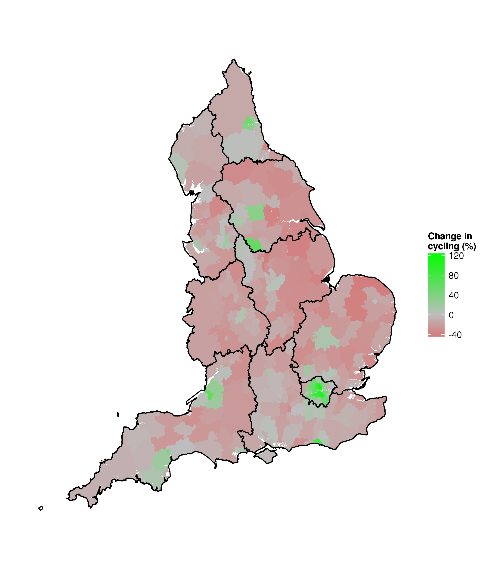
\includegraphics{figure/unnamed-chunk-5.png}
\caption{Scatter plot matrix showing distributions and relationships
between the variables of the baseline model}
\end{figure}

\subsection{Additional variables}\label{additional-variables}

In addition to these baseline input datasets, a number of other
variables were tested to investigate the relationship between other
variables and cycling to work. These were, in order that they were
tested:

\begin{itemize}
\itemsep1pt\parskip0pt\parsep0pt
\item
  The proportion of trips made by car in 2001 ($pCar$)
\item
  The change in the proportion of young (18 - 39), white males in each
  area, 2001 to 2011 ($\Delta pYWM$), following Parkin et al. (2008) who
  found this to be an important explanatory variable.
\item
  The number of cars per household in 2001 ($carOwn$) and change in car
  ownership ($\Delta carOwn$)
\end{itemize}

\section{Method}\label{method}

In line with the principle of parsimony, the modelling approach was to
start simply, by reporting key statistics about changes in cycle
commuting in England, before progressing to a regression model.

The proportion of people cycling to work (\emph{pCycle}) was calculated
as the total number of bicycle commuters ($Cycle$) divided the number of
people commuting by all modes ($Commute$) for each area ($a$). At the
national level, this can be represented as the population-weighted sum
of \emph{pCycle} for all areas:

\[PCycle =  \frac{\sum_{a=1}^n pCycle_a Commute_a}{\sum_{a=1}^n Commute_a} \]

where $PCycle$ is the proportion cycling overall and $pCycle_a$ is the
proportion cycling in each area. This is expressed more concisely as the
total number of cyclists divided by the total number of commuters
($PCycle = Cycle / Commute$). However, the above equation is useful in
demonstrating how a single national value can mask substantial regional
variation and highlights the importance of a zone's total population:
while the \emph{average} value of \emph{pCycle} dropped from 3.3 to
3.1\% across English LAs from 2001 to 2011, \emph{PCycle} remained
constant. In other words cycling grew in the (urban) LAs with higher
than average populations.

The categories of ``unemployed'' and ``work from home'' were
deliberately excluded from the $Commut$ count, to prevent changes in
employment structure influencing the result: if a commuter belt shifted
away from car driving towards `teleworking' (working from home), for
example, this method could provide an unfairly optimistic impression of
the uptake of cycling.

The dependent variable, \emph{change} in the proportion of people
cycling to work, can be defined in two ways. First, the \emph{absolute
difference} in the percentage of people cycling to work
($\Delta pCycle$) was calculated by subtracting the 2011 results from
the 2001 results. Second, \emph{relative change} ($Q pCycle$) was
defined as proportion of people cycling in 2011 divided by the rate in
2001.

A linear regression model was used to test the impact of the explanatory
variables on model fit, and to elucidate the direction of influence.
Following the principle of parsimony in model design, a simple model
based on the hypotheses presented in the introduction was developed
first. Against this baseline the performance of different model runs was
compared. To this end the following alterations were made:

\begin{itemize}
\itemsep1pt\parskip0pt\parsep0pt
\item
  Changes to the number and type of explanatory variables used.
\item
  Subsetting the observations used for the model (e.g.~to exclude
  London)
\item
  Altering the dependent variable itself to explore the relationship
  between absolute and relative increases in cycling.
\end{itemize}

\section{Results}\label{results}

The rate of cycling between 2001 and 2011 census was found to have
changed very little, being 3.1\% in both cases. However, there was
substantial variation between the zones in terms of change in cycling.
There is a strong positive skew in the distribution the growth rate
(fig. 3): less than a quarter (74) of LAs saw the modal share of cycling
rise, by an average of 30\% whereas the majority of LAs (250) saw small
declines in the proportion of people cycling.

In terms of absolute growth, the distribution is more symmetrical, with
the vast majority of zones (264 zones, 81\%) seeing less than a 1\%
change either way in absolute proportion of people cycling to work.
These results are plotted geographically in fig. 4.

\begin{figure}[htbp]
\centering
% 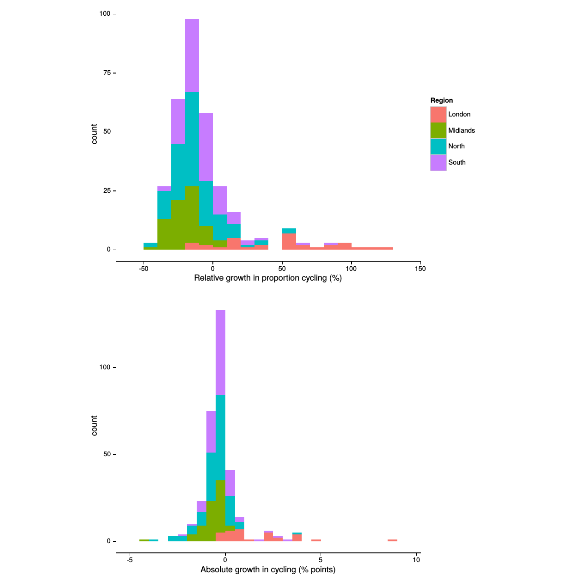
\includegraphics{figure/unnamed-chunk-6.png}
\caption{Histograms of the distribution in the growth in cycling in
absolute (above) and relative (below) terms}
\end{figure}

\begin{figure}[htbp]
\centering
% 
\includegraphics{figure/unnamed-chunk-7.png}
\caption{Change in proportion of cycle commuters in England, 2001 to
2011}
\end{figure}

It is interesting to note that the average cycling rate in 2001 was
lower for zones where cycling dropped (3.3 \%) compared with zones where
cycling grew (3.7\%). Indeed, the variability in the proportional of
people cycling grew between 2001 and 2011, despite the mean remaining
the same: the standard deviation increased from 2.5 percentage points in
2001 to 2.7 in 2011. At the MSOA level the standard deviation of the
percentage of people cycling to work also grew noticeably, from 2.7 to
2.9.

Far from cycling becoming more accessible to everyone everywhere, these
results provide some geographical evidence for a divergence between the
cycling `haves' and `have nots'. Spatial inequality in cycling as a mode
of travel to work in recent years in England, supporting the hypothesis
of positive feedback loops in modal shift to cycling through `strength
in numbers' and the normalisation of cycling culture
(borjesson2012benefits, goetzke2011bicycle).

The regional distribution of growth in cycling, with its focus on
London, is also evident from fig 5, which shows the expected high
correlation between the percent cycling to work in 2001 and 2011
(r-squared = 0.82). The $x = y$ line in fig x represents the `break
even' point above which cycling has grown and below which it has
dropped. Thus, there are 74 points above the line and the rest fall
below. The further points are located from this break even line the more
cycling has changed in that area. The colours illustrate that many of
the zones with the greatest growth in cycling are located within the
Greater London Authority.

\begin{figure}[htbp]
\centering
% 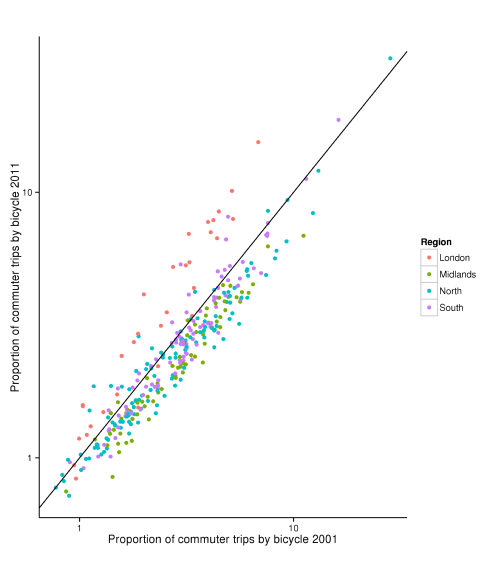
\includegraphics{figure/unnamed-chunk-8.png}
\caption{Scatterplot of the proportion of commuters who report using a
bicycle as their main means of travel to work in 2001 (x axis) and 2011
(y axis). Colours correspond to English regions.}
\end{figure}

The regional pattern represented by the colours in fig. 5 is emphasised
in Table 1, which shows that outside London there were falls in the
proportion of people cycling to work, with the greatest declines in the
Midlands and the North: the average LA in the Midlands saw the
proportion of people cycling to work drop by a fifth.

Table 1: regional differences in the change in cycling as a commuter
mode in England, 2001 to 2011.

\begin{longtable}[c]{@{}lrr@{}}
\toprule\addlinespace
Region & Relative change & Absolute change
\\\addlinespace
\midrule\endhead
London & 47.4 & 1.6
\\\addlinespace
Midlands & -19.7 & -0.7
\\\addlinespace
North & -12.3 & -0.5
\\\addlinespace
South & -7.8 & -0.2
\\\addlinespace
\bottomrule
\end{longtable}

Because of this apparent ``London exceptionalism'', the analysis was
re-run with London removed. It was found that outside London, the
proportion of all people cycling to work dropped substantially, from
3.2\% in 2001 to 2.9\% in 2011. \emph{The average LA outside London saw
a 12\% drop in the proportion of people cycling}. These results suggest
that attempts to `get Britain cycling' have so far failed outside of the
capital, which has seen the country's only large `congestion charge'
scheme encourage active travel (nakamura2014economic).

Some urban areas outside London broke the trend, seeing cycling as a
mode of travel to work grow, yet only in 12 zones did the cycling to
work increase by more than half a percentage point. (These were, in
descending order of growth rate, were Cambridge, Bristol, Oxford,
Brighton, Exeter, Newcastle, South Cambridgeshire, South
Gloucestershire, Manchester, Sheffield and Bournemouth.) Of these, only
5 had growth rates above 1 percent. In the name of balance, it was
decided to focus equally on the areas where cycling has fallen greatly:
there is a tendency towards picking `best case' studies in the cycling
literature. This can be seen as analogous to the disproportionate
non-publication of medical trials that have negative results: it is
important to focus on `failures' as well as `success stories' to provide
impartial evidence to policy makers
(\href{http://www.bmj.com/content/347/bmj.f6104?tab=citation}{Jones et
al., 2013}).

Table 2 presents the growth in cycling in the top 5 and bottom 5 areas
in terms of absolute shift in the proportion of people cycling to work.
It is noticeable that while 4 of the top 5 received central government
funding between 2001 and 2011 from the CDT initiative, none of the
bottom 5 did. (Oxford is conspicuously missing from the list of CDT
beneficiaries, and some cycle campaigners have accused the local council
of failing to properly maintain the city's existing cycle infrastructure
(\href{http://www.oxfordmail.co.uk/news/2296153.print/}{Horne, 2008}).)
This suggests that, in addition to investment helping to increase the
rate of cycling, it can also serve to maintain it and prevent declines
in areas that have an already high rate of cycling.

Table 2: Statistics on cycle commuting from the top 5 and bottom 5 local
authorities in England in terms of the absolute change in the proportion
of commuters cycling to work. Note that `CDT' refers to central
government funding through Cycling Demonstration towns and the value is
the year in which the funding was awarded.

\begin{longtable}[c]{@{}lrrrrl@{}}
\toprule\addlinespace
Local Authority & pCycle 2001 & pCycle 2011 & $\Delta pCycle$ &
$Q pCycle$ & CDT
\\\addlinespace
\midrule\endhead
Cambridge & 28.3 & 31.9 & 3.6 & 12.7 & 2009
\\\addlinespace
Bristol, City of & 4.9 & 8.1 & 3.1 & 63.7 & 2009
\\\addlinespace
Oxford & 16.2 & 18.7 & 2.5 & 15.5 & No
\\\addlinespace
Brighton and Hove & 3.0 & 5.3 & 2.4 & 80.1 & 2005
\\\addlinespace
Exeter & 4.8 & 6.6 & 1.8 & 37.3 & 2005
\\\addlinespace
& & & & &
\\\addlinespace
:---------------------------- & ---------: & -------: & -----------: &
-------: & :---------
\\\addlinespace
Boston & 11.1 & 6.9 & -4.3 & -38.4 & No
\\\addlinespace
Hull & 12.3 & 8.3 & -4.0 & -32.2 & No
\\\addlinespace
Waveney & 9.3 & 6.5 & -2.7 & -29.6 & No
\\\addlinespace
Fenland & 7.4 & 4.9 & -2.6 & -34.4 & No
\\\addlinespace
North East Lincolnshire & 8.2 & 5.6 & -2.6 & -31.2 & No
\\\addlinespace
\bottomrule
\end{longtable}

\subsection{Regression model results}\label{regression-model-results}

The baseline model was able to explain 16\% of the variation in
$\Delta pCycle$ and 14\% of the variability in $Q pCycle$ across all
zones, with adjusted R-squared ($aR^2$) values of 0.16 and 0.14
respectively. This is a statistically significant by not particularly
impressive result. In addition, the most significant variable, $Bcrash$,
had the opposite sign as expected, indicating that cycling may have
become proportionally riskier in places where cycling has grown the most
(see Table 3). Indeed, the correlation between $Bcrash$ and
$\Delta pCycle$ was strongly positive (r = 0.31).

We can speculate why this may be - perhaps car drivers in growth areas
were relatively unused to high cyclist volumes or perhaps accident rates
are higher amongst new cyclists. Yet correlation does not prove
causality and the number of cycle commuters is a poor indication of
\emph{exposure}, meaning that the results do not show with any certainty
that cycling really did tend to become less safe in areas where cycling
grew. It is implausible to assume that growth in cycling was
\emph{caused} by the increase in \emph{Bcrash} (although the reverse may
be true), so this variable was removed from subsequent model runs.

$Avinc$ and $CDT$ had a statistically significant (p \textless{} 5\%)
impact on $\Delta pCycle$ in the baseline model in the direction
expected. $Avinc$ had a strong positive correlation with $\Delta pCycle$
(r = 0.22) and $Q pCycle$ (r = 0.21). Despite there being only 17 CTD
projects (their impact spread across 19 LAs), the impact on the model
was statistically significant: CDT funding increased the proportion of
people cycling in an LA by on average 0.6 \% points in the baseline
model. To explain a greater proportion of the variability in change in
cycling to work, the additional variables were added in place of
\emph{Bcrash}.

Table 3: Results from the baseline model.

\begin{longtable}[c]{@{}lrrrr@{}}
\toprule\addlinespace
Variable & Estimate & Std. Error & t value & P
\\\addlinespace
\midrule\endhead
(Intercept) & -2.32 & 0.33 & -7.1 & 0.00
\\\addlinespace
Avinc & 0.00 & 0.00 & 4.3 & 0.00
\\\addlinespace
Lpath & -28.08 & 26.88 & -1.0 & 0.29
\\\addlinespace
Bcrash & 3.91 & 0.71 & 5.5 & 0.00
\\\addlinespace
CDT & 0.61 & 0.25 & 2.4 & 0.02
\\\addlinespace
\bottomrule
\end{longtable}

\subsection{Additional variables}\label{additional-variables-1}

Adding more variables improved the model fit. With $Bcrash$ removed, the
additional variables mentioned in the Data section were tested one by
one. The variable that had by far the greatest impact on the model was
the proportion of trips made by car drivers in 2001. Replacing $Bcrash$
with \emph{pCar} in the baseline model meant that half of the variation
in $\Delta pCycle$ could be explained, rising to 2/3 when $Q pCycle$ was
predicted ($aR^2$ 0.50 and 0.66, respectively).

Replacing $pCar$ with $\Delta pYWM$ led to a poorer model fit, although
the variable had a statistically significant impact on the model at the
5\% level in the expected positive direction as a predictor of
$Q pCycle$. $\Delta carOwn$ also had a minimal effect on the model at
this stage.

\subsection{Removing London}\label{removing-london}

As can be seen in fig. 5, LAs within London had anomalously high growth
rates, some of which can be explained by factors exclusive to the
capital such as the congestion charge, slow traffic speeds and an influx
of young, mobile workers. A strong case can thus be made for treating
London separately. When London was removed, this had a large impact on
the baseline model: the \emph{p} value of \emph{CDT} fell dramatically,
from 0.02 in the baseline model to less than 1 in 100,000 with London
excluded. In addition the slope of the estimated impact of CDT funding
increased to 0.8\% points.

With London removed, the influence of $\Delta pCar$ dropped
substantially although it was still highly statistically significant in
the expected direction. The impacts of the other additional variables
were statistically insignificant.

\subsection{The final model}\label{the-final-model}

The simplest solution that explained a high proportion of variability in
cycling to work was chosen. This was found to be the following
expression:

\[Q pCycle \sim Avinc + pCar +  CDT \]

Across all Local Authorities, this model accounts for 2/3 of the change
in cycling. However, the final model results presented in Table 4
exclude London LAs which were deemed to be anomalous. This final model
explains roughly 1/3 of the change in the rate of cycling ($aR^2$ =
0.27) based on only 3 variables, all of which are significant at the 5\%
level. As before, $pCar$ was the most powerful explanatory factor.

Table 4: Results from the final model

\begin{longtable}[c]{@{}lrrrr@{}}
\toprule\addlinespace
Variable & Estimate & Std. Error & t value & P
\\\addlinespace
\midrule\endhead
(Intercept) & 55.825 & 8.783 & 6.356 & 0.000
\\\addlinespace
Avinc & 0.032 & 0.008 & 4.178 & 0.000
\\\addlinespace
pCar & -134.211 & 14.078 & -9.534 & 0.000
\\\addlinespace
CDT & 6.803 & 3.424 & 1.987 & 0.048
\\\addlinespace
\bottomrule
\end{longtable}

\section{Discussion}\label{discussion}

Cycling for personal transport has become more unequal over space in the
last 10 years: most of the growth in cycle commuting has happened in
London and a few urban centres outside the capital. This coincides with
findings of geographical divergence of many other geographic variables
related to health and the economy (Dorling, 2011). Excluding London from
the analysis, cycle commuting has declined overall from 3.2 to 2.9\% of
trips. Within this aggregate figure, a few areas have seen very
impressive rates of growth in cycling and a number of these received
central government funding through the Cyclind Development Towns
project. Yet the trend for a typical English LA outside London has been
decline: the median value of pCycle dropped by 0.4\% points from 2.9 to
2.5\%, a worrying trend about which many academics and cycle campaigners
seem unaware.

That is not to downplay the success stories, but raises the question:
why did cycle commuting in some areas grow against a backdrop of
decline? The paper has been able to provide some answers here: areas
with high incomes, historically low rates of car use and government
support have tended to do well. This does not prove cause and effect: it
is plausible to suggest that areas received cycle funding precisely
because they were seen as success stories.

Returning to the hypotheses posed in the introduction, we have provided
statistically significant evidence that the health and other benefits of
cycling are disproportionately being enjoyed in high income areas, where
much of the growth has occurred. No significant evidence about the
positive influence of safe roads or bicycle path provision was found.
More research is needed in both areas and the study has by no means
disproved a link.

The findings support previous calls for more rigorous studies exploring
the impact of different environments and policies on active travel
(Fraser and Lock, 2011). Specifically, there is a need for a database on
public expenditure on cycling and an up-to-date database on cycle paths
and other pro-cycling features. Only with official high quality
databases (or improvements in Open Street Map) will we able to compare
the impacts of different interventions.

There are a number of limitations to the study. Using areal units to
explain any issue that is ultimately played out at the individual level
risks committing the `ecological fallacy': falsely inferring things
about individuals based on aggregated data (Openshaw, 1983). To avoid
this problem we have been careful to state that the findings apply only
to areas and not necessarily to the citizens who occupy them. We cannot
know from the results, for example, that individuals on high incomes are
tending to cycle more, just that the number of people reporting cycling
to work in areas with high average incomes has grown. There is, however,
verbal evidence of the importance of class and cultural identity in the
context of cycling growth in wealthy areas (Aldred and Jungnickel,
2014), with which our results coincide.

The research presented in this paper also raises important questions
about data quality. From a health perspective, the number of people who
use bicycles as their \emph{main} form of transport to work is far less
important than the number of people who cycle once or twice per week.
The marginal benefit of exercise decreases after a few hours of moderate
exertion per week and a roughly typical cycle commute of 3 miles each
way could easily reach this amount. More important from a health
perspective (and potentially from an environmental perspective) is the
number of people who \emph{sometimes} cycle to work, once or twice per
week, but not always. Because cycling is often a `plan B' mode to be
used occasionally, the potential impact of under-reporting of trips is
large. Conversely, there may be many people who entered cycling as their
primary mode of transport to work as `aspirational cyclists' who cycle
occasionally but would like to think that they always do. These
questions of data quality require further analysis and the National
Travel Survey could provide a useful empirical starting point for future
research into this area.

In terms of monitoring the geographical distribution of a shift to
cycling, a more suitable independent variable would be the total number
of trips taken by residents of each area per year. Even more
specifically, estimates of the total distance cycled in each area, and
the social distribution of this cycling activity across society as a
whole would be preferable. Indeed, if cycling is concentrated amongst
healthy men, it is realising only a fraction of the potential health
benefits.

\section{Conclusion}\label{conclusion}

This study provides new evidence about the spatial distribution of
uptake and declines in cycling to work across England. Regression
analysis at the level of Local Authorities was used to test hypotheses
about factors expected to be associated with growth in cycling. Of
these, statistically significant results were found for average income
and government support for cycling at the level of local authorities.
The former supports the wider `peak car' narrative (Goodwin and Van
Dender, 2013). Perhaps more relevant for local policy makers is the
latter - that cycling grew significantly \emph{more} in areas which
received central government funding through CDTs. This supports
additional tranches of central government funding for cycling,
especially targetting low income areas.

The study uses \emph{change} in the rate of cycling to work over 10
years as the dependent variable. This differs from most geographical
studies on the subject, which generally explain cycling variability at
one specific point in time (e.g.~Parkin et al., 2008). These studies
focus attention on variables that are either inherent to the natural
environment (e.g.~topology, weather) or which are not easy to alter
through policy interventions (e.g.~average distance of trips) (Fraser
and Lock, 2011).

Amongst these factors, average income was found to be most strongly
associated with cycling, providing further evidence that growth in
cycling has been driven in recent years primarily by the wealthy
(Goodman, 2013). This coincides with evidence from the `peak car'
literature that high income groups are tending to drive less each year
(Metz 2013). Of course, the average income of people in different areas
is a factor outside the control of most policy makers (although they may
wish otherwise). Yet the finding is important in terms of policy design
as it provides additional evidence that more needs to be done to promote
cycling amongst the most disadvantaged in society (Christie, 2011). The
study supports the conclusion that ``care needs to be taken to also
develop interventions in lower-income areas'' (Aldred and Jungnickel,
2014).

An unexpected finding that merits further analysis was that the most
powerful predictor of change in cycling was the proportion of people
driving to work in 2001. We can speculate about why this may be. The
result may be linked to confounding factors such as average distances
between home and work locations, for example. In any case strength of
the relationship supports the idea that cars and bicycles can be seen in
ecological terms as `species' in direct competition (Lovelace et
al.,2011). The policy implication of this finding is that in some cases
the best way to promote active travel from a health perspective may be
to implement policies discouraging car use (Jacobsen et al., 2009).

The limitations of the study relate to its methodology and use of
administrative zones as the unit of analysis. Focussing on reported
cycling to work as the dependent variable is problematic because cycling
to work is not an either/or decision but something that can vary widely,
from every day to a few times per month (Stinson and Bhat, 2004). Such
subtleties are simply not collected in the Census: there is a trade-off
between geographic resolution and coverage from census data and depth
and insight from individual-level surveys. The paper therefore advocates
further studies that seek to integrate detailed survey datasets with
information from the Census, for example by comparing correlations
between Census and individual level variables (Goodman, 2013) or more
complex techniques such as spatial microsimulation (Lovelace et
al.,2014).

It is clear that more research is needed on how best to promote cycling.
Returning to the global issues raised in the introduction, we have
demonstrated that, in addition to improved data on the \emph{problems},
there is also mounting of evidence about potential \emph{solutions}.
Policies to promote cycling represent one option amongst many, but their
simplicity and low cost make them ideally suited to the current context
of risk aversion and austerity. Interventions that increase cycling are
also exceptional in the wide range of interrelated problems they tackle.
Health and environmental impacts can be seen as unintentional
`co-benefit' of improving the performance transport systems.

Investment in cycling is a cost effective way to pursue sustainability,
with proven health benefits. There is a limited time window in which
still abundant physical and economic resources can be spent on a
sustainable future, so measures should be pursued with some urgency. For
cycling investment to be effective, however, policies need to be based
on evidence: about what works, what does not and where funding is likely
to have the greatest health and environmental benefits. The findings of
this paper cannot prescribe policies. Interpreted with care and
intelligence, they can help ensure that specific measures are
implemented where they are most needed.

\section{References}\label{references}

Aldred, R., \& Jungnickel, K. (2014). Why culture matters for transport
policy: the case of cycling in the UK. Journal of Transport Geography,
(early), 1--22. Retrieved from
http://www.sciencedirect.com/science/article/pii/S0966692313002202
Arnott, R., Rave, T., \& Schöb, R. (2005). Alleviating urban traffic
congestion. MIT Press Books, 1.

Beddoe, R., Costanza, R., Farley, J., Garza, E., Kent, J., Kubiszewski,
I., \ldots{} Woodward, J. (2009). Overcoming systemic roadblocks to
sustainability: The evolutionary redesign of worldviews, institutions,
and technologies. Proceedings of the National Academy of Sciences,
106(8), 2483--2489. doi:10.1073/pnas.0812570106

Berners-Lee, M., \& Clark, D. (2013). The Burning Question: We can't
burn half the world's oil, coal and gas. So how do we quit? (p.~256).
Profile Books.

Börjesson, M., \& Eliasson, J. (2010). The value of time and external
benefits in bicycle cost-benefit analysEs. In Proceedings of the 12th
World Conference on Transport Research (WCTR) (pp.~11--15).

Cifuentes, L., Borja-Aburto, V. H., Gouveia, N., Thurston, G., \& Davis,
D. L. (2001). Hidden Health Benefits of Greenhouse Gas Mitigation.
Science, 293(5533), 1257--1259. doi:10.1126/science.1063357

Dorling, D. (2011). Injustice: Why social inequality persists. The
Policy Press.

Downs, A. (2011). Still stuck in traffic. Brookings Institute Press.
Washington DC.

Ehrlich, P. R., \& Ehrlich, A. H. (2013). Can a collapse of global
civilization be avoided? Proceedings of the Royal Society B: Biological
Sciences, 280(1754).

Fishman, E., Washington, S., \& Haworth, N. (2013). Bike Share: A
Synthesis of the Literature. Transport Reviews, 33(2), 148--165.
doi:10.1080/01441647.2013.775612

Fraser, S. D. S., \& Lock, K. (2011). Cycling for transport and public
health: a systematic review of the effect of the environment on cycling.
European Journal of Public Health, 21(6), 738--43.
doi:10.1093/eurpub/ckq145

Furness, Z. (2010). One less car: Bicycling and the politics of
automobility. Temple University Press.

Goodman, A. (2013). Walking, Cycling and Driving to Work in the English
and Welsh 2011 Census: Trends, Socio-Economic Patterning and Relevance
to Travel Behaviour in General. PLoS ONE, 8(8), e71790.
doi:10.1371/journal.pone.0071790

Gray, D., Farrington, J., Shaw, J., Martin, S., \& Roberts, D. (2001).
Car dependence in rural Scotland: transport policy, devolution and the
impact of the fuel duty escalator. Journal of Rural Studies, 17(1),
113--125. doi:10.1016/S0743-0167(00)00035-8

Gross, R., Heptonstall, P., Anable, J., \& Greenacre, P. (2009). What
policies are effective at reducing carbon emissionsfrom surface
passenger transport ? Retrieved from
http://www.ukerc.ac.uk/support/TransportReport

Hansen, M. H., \& Yu, B. (2001). Model Selection and the Principle of
Minimum Description Length. Journal of the American Statistical
Association, 96(454), 746--774. doi:10.1198/016214501753168398

Horne, D. (2008). £4m snub to city cyclists (From Oxford Mail). Oxford
Mail. Retrieved May 24, 2014, from
http://www.oxfordmail.co.uk/news/2296153.print/

Hughes, J. D. (2013). Energy: A reality check on the shale revolution.
Nature, 494(7437), 307--308. Retrieved from
http://dx.doi.org/10.1038/494307a

Jacobsen, P. L., Racioppi, F., \& Rutter, H. (2009). Who owns the roads?
How motorised traffic discourages walking and bicycling. Injury
Prevention : Journal of the International Society for Child and
Adolescent Injury Prevention, 15(6), 369--73. doi:10.1136/ip.2009.022566

Jarrett, J., Woodcock, J., Griffiths, U. K., Chalabi, Z., Edwards, P.,
Roberts, I., \& Haines, A. (2012). Effect of increasing active travel in
urban England and Wales on costs to the National Health Service. Lancet,
379(9832), 2198--205. doi:10.1016/S0140-6736(12)60766-1

Komanoff, C. (2004). Bicycling. In J. C. Cutler (Ed.), Encyclopedia of
Energy (pp.~141--150). New York: Elsevier.

Lenzen, M. (1999). Total requirements of energy and greenhouse gases for
Australian transport. Transportation Research Part D: Transport and
Environment, 4(4), 265--290. doi:DOI: 10.1016/S1361-9209(99)00009-7

Lewis, N. S., \& Nocera, D. G. (2006). Powering the planet: chemical
challenges in solar energy utilization. Proceedings of the National
Academy of Sciences of the United States of America, 103(43), 15729--35.
doi:10.1073/pnas.0603395103

Lindsay, G., Macmillan, A., \& Woodward, A. (2011). Moving urban trips
from cars to bicycles: impact on health and emissions. Australian and
New Zealand Journal of Public Health, 35(1), 54--60.
doi:10.1111/j.1753-6405.2010.00621.x

Lovelace, R. (2014). The energy costs of commuting: a spatial
microsimulation approach. University of Sheffield. Retrieved from
http://etheses.whiterose.ac.uk/5027/

Lovelace, R., Beck, S. B. M. B. M., Watson, M., \& Wild, A. (2011).
Assessing the energy implications of replacing car trips with bicycle
trips in Sheffield, UK. Energy Policy, 39(4), 2075--2087.
doi:10.1016/j.enpol.2011.01.051

McMillan, M., Shepherd, A., Sundal, A., Briggs, K., Muir, A., Ridout,
A., \ldots{} Wingham, D. (2014). Increased ice losses from Antarctica
detected by CryoSat-2. Geophysical Research Letters, n/a--n/a.
doi:10.1002/2014GL060111

Michaelowa, A., \& Dransfeld, B. (2008). Greenhouse gas benefits of
fighting obesity. Ecological Economics, 66(2-3), 298--308.
doi:10.1016/j.ecolecon.2007.09.004

Nutley, S. (1980). Accessibility, mobility and transport-related
welfare: the case of rural Wales. Geoforum, 11(1977), 335--352.
Retrieved from
http://www.sciencedirect.com/science/article/pii/0016718580900226

Oja, P., Titze, S., Bauman, a, de Geus, B., Krenn, P., Reger-Nash, B.,
\& Kohlberger, T. (2011). Health benefits of cycling: a systematic
review. Scandinavian Journal of Medicine \& Science in Sports, 21(4),
496--509. doi:10.1111/j.1600-0838.2011.01299.x

Openshaw, S. (1983). The modifiable areal unit problem. Group. Geo Books
Norwich,, UK. Retrieved from http://www.getcited.org/pub/102412488

Parkin, J., Wardman, M., \& Page, M. (2008). Estimation of the
determinants of bicycle mode share for the journey to work using census
data. Transportation, 35(1), 93--109. doi:10.1007/s11116-007-9137-5

Prime Minister's Office, \& Department for Transport. (2013). Government
shifts cycling up a gear - press release. Press release. Retrieved
September 26, 2013, from
https://www.gov.uk/government/news/government-shifts-cycling-up-a-gear

Pucher, J., \& Buehler, R. (2008). Making Cycling Irresistible: Lessons
from The Netherlands, Denmark and Germany. Transport Reviews, 28,
495--528.

Pucher, J., Dill, J., \& Handy, S. (2010). Infrastructure, programs, and
policies to increase bicycling: An international review. Preventive
Medicine, 50(Supplement 1), S106 -- S125. doi:DOI:
10.1016/j.ypmed.2009.07.028

Robinson, D. L. (2005). Safety in numbers in Australia: more walkers and
bicyclists, safer walking and bicycling. Health Promotion Journal of
Australia: Official Journal of Australian Association of Health
Promotion Professionals, 16(1), 47--51. Retrieved from
http://www.ncbi.nlm.nih.gov/pubmed/16389930

Rojas-Rueda, D., \& Nazelle, A. De. (2011). The health risks and
benefits of cycling in urban environments compared with car use: health
impact assessment study. BMJ, 1--8. doi:10.1136/bmj.d4521

Rutter, H., Cavill, N., Racioppi, F., Dinsdale, H., Oja, P., \&
Kahlmeier, S. (2013). Economic impact of reduced mortality due to
increased cycling. American Journal of Preventive Medicine, 44(1),
89--92. doi:10.1016/j.amepre.2012.09.053

Schweizer, J., \& Rupi, F. (2014). Performance Evaluation of Extreme
Bicycle Scenarios. Procedia - Social and Behavioral Sciences, 111,
508--517. doi:10.1016/j.sbspro.2014.01.084

Sexton, S., Wu, J. J., \& Zilberman, D. (2012). How High Gas Prices
Triggered the Housing Crisis: Theory and Empirical Evidence. In Press.
Retrieved from
http://www.chikyu.ac.jp/archive/topics/2011/111219\_JunJieWu.pdf

Sheehan, J. J. (2009). Biofuels and the conundrum of sustainability.
Current Opinion in Biotechnology, 20(3), 318--324.
doi:http://dx.doi.org/10.1016/j.copbio.2009.05.010

Smil, V. (2008). Energy in nature and society (p.~495). MIT Press.

Sustrans. (2012). Locked out: transport poverty in England (p.~2).
Bristol.

Titheridge, H., \& Hall, P. (2006). Changing travel to work patterns in
South East England. Journal of Transport Geography, 14(1), 60--75.
doi:10.1016/j.jtrangeo.2005.06.006

Woodcock, J., Edwards, P., Tonne, C., Armstrong, B. G., Ashiru, O.,
Banister, D., \ldots{} Roberts, I. (2009). Public health benefits of
strategies to reduce greenhouse-gas emissions: urban land transport. The
Lancet, 374(9705), 1930--1943. doi:10.1016/S0140-6736(09)61714-1
